\documentclass[11pt,a4paper]{report}
\usepackage[margin=1in]{geometry}
\geometry{top=1.3in,headheight=41pt,headsep=12pt}
\usepackage[T5,T1]{fontenc}
\usepackage[utf8]{inputenc}
\usepackage{graphicx}
\usepackage{fancyhdr}
\usepackage{lastpage}
\usepackage{amsmath,amssymb}
\usepackage{tikz}
\usepackage{tikz-cd}
\usetikzlibrary{arrows.meta,positioning,calc,shapes.geometric}
\usepackage{multicol}
\usepackage{array,booktabs,tabularx}
\usepackage{longtable}
\usepackage{enumitem}
\usepackage{microtype}
\usepackage{caption}
\usepackage{xurl}
\usepackage[hidelinks,hypertexnames=false]{hyperref}
\hypersetup{pdftitle={Thesis Deposit System on the DSpace Digital Library},
  pdfauthor={Nguyen Tran Huu Duc; Bui Vu Thien Dang; Nguyen Phuc Nhan}}
\newcommand{\code}[1]{{\small\texttt{\detokenize{#1}}}}
\newcolumntype{Y}{>{\raggedright\arraybackslash}X}
\renewcommand{\bibname}{References}
\captionsetup{font=small,labelfont=bf}
\emergencystretch=2em
\setlength{\tabcolsep}{5pt}
\renewcommand{\arraystretch}{1.15}

\setlength{\headheight}{41pt}
\pagestyle{fancy}
\fancyhf{}
\fancyhead[L]{%
  \begin{tabular}{@{}rl@{}}
    \includegraphics[width=10mm,height=10mm,keepaspectratio]{\detokenize{report-assets/hcmut.png}} &
    \begin{tabular}{@{}l@{}}
      \small\textbf{Ho Chi Minh City University of Technology - VNU-HCM}\\
      \small\textbf{Faculty of Computer Science and Engineering}
    \end{tabular}
  \end{tabular}%
}
\fancyhead[R]{}
\fancyfoot[L]{\scriptsize Specialized Project Report}
\fancyfoot[R]{\scriptsize Page \thepage}
\renewcommand{\headrulewidth}{0.3pt}
\renewcommand{\footrulewidth}{0.3pt}
\fancypagestyle{plain}{%
  \fancyhf{}
  \fancyhead[L]{%
    \begin{tabular}{@{}rl@{}}
      \includegraphics[width=10mm,height=10mm,keepaspectratio]{\detokenize{report-assets/hcmut.png}} &
      \begin{tabular}{@{}l@{}}
        \small\textbf{Ho Chi Minh City University of Technology - VNU-HCM}\\
        \small\textbf{Faculty of Computer Science and Engineering}
      \end{tabular}
    \end{tabular}%
  }
  \fancyhead[R]{}
  \fancyfoot[L]{\scriptsize Specialized Project Report}
  \fancyfoot[R]{\scriptsize Page \thepage}
  \renewcommand{\headrulewidth}{0.3pt}
  \renewcommand{\footrulewidth}{0.3pt}
}

\setlength{\parindent}{0pt}
\setlength{\parskip}{0.55\baselineskip}
\setlist[itemize]{leftmargin=1.6em,itemsep=0.15em,topsep=0.25em}
\setlist[enumerate]{leftmargin=1.8em,itemsep=0.15em,topsep=0.25em}

\begin{document}

\begin{titlepage}
\begin{tikzpicture}[remember picture, overlay]
  \draw[line width=4pt]
    ($(current page.north west) + (0.4in,-0.5in)$)
    rectangle
    ($(current page.south east) + (-0.4in,0.5in)$);
  \draw[line width=1.5pt]
    ($(current page.north west) + (0.45in,-0.55in)$)
    rectangle
    ($(current page.south east) + (-0.45in,0.55in)$);
\end{tikzpicture}
\thispagestyle{empty}
\centering
\begingroup
\setlength{\parskip}{0pt}
\vfill
{\large\bfseries
VIETNAM NATIONAL UNIVERSITY, HO CHI MINH CITY\\
HO CHI MINH CITY UNIVERSITY OF TECHNOLOGY\\
FACULTY OF COMPUTER SCIENCE AND ENGINEERING\par}
\vfill
\includegraphics[width=1.9in]{\detokenize{report-assets/hcmut.png}}\par
\vfill
{\Large\bfseries REPORT\\
SPECIALIZED PROJECT\par}
\vfill
{\rule{0.8\textwidth}{0.6pt}\par}
\vfill
{\LARGE\bfseries
THESIS DEPOSIT SYSTEM\\
ON THE DSPACE\\
DIGITAL LIBRARY\par}
\vfill
{\rule{0.8\textwidth}{0.6pt}\par}
\vfill
{\Large\bfseries MAJOR: COMPUTER SCIENCE\par}
\vfill
{\normalsize
\begin{tabular}{@{}r@{\,:\,}l@{}}
  \textbf{SUPERVISOR} & MSc. Nguyen Cao Tri \\
  \textbf{COURSE CODE} & CO4029 - HK261-DAGD1-062
\end{tabular}\par}
\vfill
{\large\bfseries ---------o0o---------\par}
\vfill
{\normalsize
\begin{tabular}{@{}r@{\,:\,}l@{}}
  \textbf{STUDENT} &
    \begin{tabular}[t]{@{}l@{}}
      Nguyen Tran Huu Duc - 2252167\\
      Bui Vu Thien Dang - 2252151\\
      Nguyen Phuc Nhan - 2252563
    \end{tabular}
\end{tabular}\par}
\vfill
{\normalsize HO CHI MINH CITY, November 2026\par}
\vfill
\endgroup
\end{titlepage}

\pagenumbering{roman}
\chapter*{Abstract}
\addcontentsline{toc}{chapter}{Abstract}
This report describes the extension of an existing electronic thesis submission portal integrated with the DSpace digital library. The inherited system provides student submission, assigned academic review, library intake, portal archival, administration, and a separate DSpace publishing operation. The present work develops a shared role-based review workspace, an authenticated embedded PDF viewer, transactional Editor metadata corrections, a Final Editor return-to-Editor loop, readable approval history, and local notification evidence. The frontend is reorganized into authentication, submissions, administration, and archive features with explicit dependency boundaries.

The implementation described here is the \code{UI-build} branch at commit \code{3d97faf3}, compared with \code{main} at \code{4f7a73df}. Recorded local evidence from 4 November 2026 reports 51 API tests, 8 email integration tests, and 12 browser tests passing. These results establish the tested portal behavior in a local environment. Digital signing, signed deposit certificates, controlled print outputs, HCMUT SSO, and a new live DSpace publication test remain outstanding integrations. The report separates these phase goals from implemented and verified behavior.
\clearpage
\tableofcontents
\clearpage
\listoffigures
\listoftables
\clearpage
\pagenumbering{arabic}


\chapter{Introduction}
\label{ch:introduction}

\section{Motivation: Electronic Thesis Deposit at HCMUT}
Electronic thesis deposit connects the student, academic reviewers, the library, and the institutional repository. Each participant needs a different view of the same submission: students need progress and correction reasons, reviewers need the assigned document and decision controls, and library staff need reliable metadata and a clear archival record. DSpace supplies the repository layer, while a separate portal can express the university's submission periods and approval process.

The preceding capstone report by Ngo Nhat Tuan describes the foundation used by this project: a React, NestJS, and PostgreSQL portal that receives thesis metadata and PDFs, coordinates review and library intake, and publishes accepted records through the DSpace REST API~\cite{previous-report}. The current project extends that foundation. It retains the existing submission and administration functions while improving how users inspect documents, correct metadata, return work for library correction, and understand the approval history.

The portal's roles are Student/Submitter, Reviewer, Library Staff, Director, and Administrator. Reviewer, Editor, and Final Editor are also used as workflow labels in the interface. They describe the portal's adaptation of DSpace workflow concepts; they do not mean that the React application is DSpace Angular or that a portal account automatically belongs to a DSpace permission group.

\begin{table}[htbp]
\centering\small
\begin{tabularx}{\textwidth}{@{}c l l Y@{}}
\toprule
\textbf{Step} & \textbf{Workflow label} & \textbf{Portal role} & \textbf{Implemented responsibility} \\
\midrule
1 & Reviewer & Reviewer & Review assigned theses; approve or reject with a reason. \\
2 & Editor & Library Staff & Inspect the PDF, correct metadata, accept or reject with a reason. \\
3 & Final Editor & Director & Return to the previous Editor with a reason, or confirm portal archival at the final step. \\
\bottomrule
\end{tabularx}
\caption{Default review-stage mapping in the current branch. Administrator is a separate configuration role.}
\label{tab:role-mapping}
\end{table}

\section{Problem Statement and Gaps in the Baseline}
The inherited portal already implements the main submission lifecycle, but the review experience and its implementation need further work. Source comparison and the branch's analysis identify five gaps~\cite{ui-report,refactoring}:
\begin{itemize}
  \item Document inspection relied on separate file access rather than a shared workspace that placed metadata and the PDF together.
  \item The Editor metadata path needed a usable form and correct persistence. In the baseline endpoint, abstract was written to description and an update referenced a column absent from the submission schema.
  \item Director rejection returned a thesis to the student. The revised requirement is a return to the previous Editor, preserving academic approvals and the existing PDF.
  \item Audit events existed but needed a consistent timeline with actor identity, role, reason, state transitions, and readable metadata changes. History access also needed submission-level authorization.
  \item Authentication, role navigation, forms, administration, and archive behavior were concentrated in large components, making changes difficult to isolate and review.
\end{itemize}

The broader phase plan additionally calls for digital signatures, electronic confirmation certificates, print controls, and future SSO and plagiarism integration. These are project requirements, but their presence in the plan does not establish that they are implemented.

\section{Objectives and Current Contribution}
The immediate objective is to make the default three-stage portal workflow usable, traceable, and consistent with the active configured step. The current branch adds a reusable task workspace, authenticated PDF.js rendering, validated partial metadata updates, a Director return loop, protected approval history, and resilient decision dialogs. A feature-based frontend structure separates session management, submissions, administration, and archive management.

The longer-term phase-1 objective remains a deposit pipeline that can sign and verify the final PDF, issue a signed confirmation certificate, provide the planned viewing/printing options, and publish the appropriate output to DSpace. Those goals require a real signing integration and a defined operational sequence before they can be reported as achieved.

\section{Scope and Implementation Status}
This report is a progress report for the current team, based on the supplied \code{main.tex} outline, the previous report, and the local repository. The comparison uses \code{main} at \code{4f7a73df} and \code{UI-build} at \code{3d97faf3}. The previous report is used as baseline context and attributed prior work; its author's declaration, authorship, and historical test outcomes are not reassigned to the present team.

\subsection*{Implemented in the current branch}
\begin{itemize}
  \item Role-oriented queues and a shared submission workspace with metadata, files, approval history, and an embedded paginated PDF preview.
  \item Editor corrections with validation, preserved omitted fields, separate abstract/description storage, synchronized queue titles, and transactional audit differences.
  \item Final Editor return-to-Editor with a required reason, retained academic approvals/files, stage checks under a row lock, and confirmation before final archival.
  \item A return notification to library staff, local Mailpit evidence, Vietnamese/English presentation, responsive views, Home navigation, and PDF rendering stability fixes.
  \item Frontend feature boundaries, static architecture checks, and a fresh-database Docker demonstration seed gated by an initialization marker.
\end{itemize}

\subsection*{Inherited facilities retained}
Student drafts/submission/resubmission, reviewer assignment, role permissions, configurable fields, local and optional Google authentication, archive hierarchy management, email settings, and the separate DSpace integration are retained. Changes to these areas are identified where the current branch extends them. Full collection-level permission synchronization with DSpace is not established by the local UI tests.

\subsection*{Planned or awaiting external validation}
PAdES signing and certificate verification, the three signature appearances, signed confirmation certificates, controlled print variants, batch signing, and a signing gate before publication are not implemented by this branch. Live DSpace publication and production email require separate current-environment validation. HCMUT SSO, plagiarism integration, a later printing stage, and additional document types remain future work. The PDF viewer currently offers authorized Open/Download access; it does not implement the planned print restrictions.

\section{Report Organization}
Chapter~2 explains the concepts needed to understand the portal. Chapter~3 identifies inherited work and the contribution boundary. Chapter~4 describes requirements, access rules, workflow, architecture, and integration contracts. Chapter~5 explains the current implementation and presents existing UI evidence. Chapter~6 records dated verification results and their limits. Chapter~7 summarizes the implemented contribution and the remaining phase work.

\clearpage\section{Team Assignment and 11-Week Plan}


The original assignment covers 28 September--13 December 2026. Table entries below are planned responsibilities, not completion claims. This report records implementation through 5 November 2026; the collected UI and test evidence is dated 4 November. Signature, printing, certificate, and later integration tasks remain planned unless explicitly identified as implemented in Chapters~\ref{ch:implementation} and~\ref{ch:evaluation}.

{\footnotesize
\renewcommand{\arraystretch}{1.1}
\setlength{\tabcolsep}{3pt}
\begin{longtable}{|>{\raggedright\arraybackslash}p{0.06\linewidth}|>{\raggedright\arraybackslash}p{0.11\linewidth}|>{\raggedright\arraybackslash}p{0.22\linewidth}|>{\raggedright\arraybackslash}p{0.22\linewidth}|>{\raggedright\arraybackslash}p{0.22\linewidth}|}
\hline
\textbf{Week} & \textbf{Dates} & \textbf{A -- Bui Vu Thien Dang (Workflow, permissions, processing pipeline)} & \textbf{B -- Nguyen Phuc Nhan (UI, viewer, testing)} & \textbf{C -- Nguyen Tran Huu Duc (E-signature, PDF output)} \\ \hline
\endfirsthead
\hline
\textbf{Week} & \textbf{Dates} & \textbf{A -- Bui Vu Thien Dang (Workflow, permissions, processing pipeline)} & \textbf{B -- Nguyen Phuc Nhan (UI, viewer, testing)} & \textbf{C -- Nguyen Tran Huu Duc (E-signature, PDF output)} \\ \hline
\endhead
\hline
\endfoot
\hline
\endlastfoot
1 & Sep 28 -- Oct 4 & Read the workflow file, reproduce the 3-step process and permission groups on the DSpace test instance & Study HCMUT's thesis deposit regulations and review the 2 existing sub-projects & Research the university's digital signature service, PAdES, and PDF signing libraries \\ \hline
2 & Oct 5 -- Oct 11 & Read the current codebase and build a gap table against DSpace & Survey the DSpace REST API (workflowitems, pooltasks, claimed tasks) & Trial-sign a PDF with a test certificate and list what information is needed from the library \\ \hline
3 & Oct 12 -- Oct 18 & Finalize the design document: state machine, role and permission matrix & Finalize the UI flow per role and the email flow & Finalize the signing approach (who signs, at which step, with what, where stored) \\ \hline
4 & Oct 19 -- Oct 25 & Change the DB schema (system roles, approval history), implement RBAC & Wireframes and task queue pages for Reviewer, Library Staff, and Director & Design the signing module, implement basic PDF signing \\ \hline
5 & Oct 26 -- Nov 1 & Workflow steps 1 and 2: Reviewer and Library Staff accept/reject with a reason; Library Staff edits metadata & UI for steps 1 and 2 (view PDF, accept/reject, metadata form); update the report outline with the supervisor & Signing core: sign a PDF, verify the signature, signature style 1 (signature strips along the page margins) \\ \hline
6 & Nov 2 -- Nov 8 & Reviewer and Library Staff reject with reasons; Director returns to Editor with a reason or archives; integrate the return flow and assess DSpace group/status alignment & UI for step 3 and the return flow, email notifications, approval history view & Signature styles 2 (diagonal across the page) and 3 (signature box), Administrator signing settings API (style, sign option), call signing when Director archives \\ \hline
7 & Nov 9 -- Nov 15 & Basic PDF validation; batch processing of existing theses (import, validate, sign); processing pipeline with hooks so later stages such as printing can be added & Administrator UI: choose the signature style with a preview, assign users to roles per collection; end-user print options UI (3 choices) & Generate the 3 print outputs (with signature, a few preview pages, blurred copy); push the signed PDF to DSpace; sign the deposit confirmation certificate \\ \hline
8 & Nov 16 -- Nov 22 & Full integration, run submission to publication end to end; unit tests for workflow and RBAC; document the extension points and API for end users who integrate later & Browser print handling: block printing, or allow printing with blurred text and a visible signature; E2E tests for Accept, Reject, and resubmit & Tests for signing, the 3 signature styles, and the 3 print outputs with various PDF types; batch signing performance \\ \hline
9 & Nov 23 -- Nov 29 & Trial run with real accounts, fix bugs, separate the authentication layer for future SSO & Trial run, polish UI, write the role-based user guide & Trial run, fix signing and print bugs, write the operations guide (certificates) and a developer guide for extending the tool \\ \hline
10 & Nov 30 -- Dec 6 & Write access control, workflow, backend implementation and evaluation sections; remaining bug fixes & Write UI, architecture, API, notification and browser evaluation sections & Write signature background, signing/output design, implementation and evaluation sections \\ \hline
11 & Dec 7 -- Dec 13 & Final report, demo preparation, phase 1 demo & Final report, demo preparation, phase 1 demo & Final report, demo preparation, phase 1 demo \\ \hline
\end{longtable}
}


\chapter{Theoretical Background}

\section{Digital Libraries and DSpace}
An institutional repository stores scholarly records and their associated files independently of the application that collected them. In this project, the portal coordinates submission and approval, while DSpace is the external repository. The inherited implementation organizes its integration around communities, collections, items, metadata, and bitstreams. A thesis PDF is transferred as a bitstream associated with a repository item; a portal submission is a separate database record.

The default portal workflow uses the labels Reviewer, Editor, and Final Editor to make the academic, library correction, and final approval responsibilities explicit. This is a project adaptation of DSpace concepts. Portal workflow execution remains in NestJS and PostgreSQL, with a distinct publishing request to DSpace. A label match alone cannot prove equivalence between portal permissions and collection-level DSpace groups.

\section{Role-Based and Submission-Level Access Control}
Role-based access control assigns capabilities to account roles. The API combines JWT authentication with permission guards and service-level checks. These layers answer different questions: whether a session is authenticated, whether its role has the relevant capability, and whether this actor may perform this operation on this submission at its present step.

Object-level checks are necessary even when the endpoint accepts a role. A reviewer can read the history of an assigned thesis, while another reviewer cannot. A coauthor can inspect an authorized record without acquiring the submitting student's mutation rights. Library staff may correct metadata only while an Editor step is active. Hiding a button in React improves the interface but does not replace these server checks.

\section{Workflow State, Transactions, and Audit History}
A workflow is defined by allowed transitions and the conditions for each transition. The portal stores the broad submission status together with the current position in a submission-specific workflow snapshot. Two records may both be \code{reviewing} while awaiting different actors; therefore the active role must be checked separately.

A state mutation and its audit event should commit together. The current implementation uses PostgreSQL transactions and locks the submission row before metadata corrections or Director return decisions. Rechecking the active step after the lock prevents a stale request from applying a decision to a stage that another request has already left. An audit trail then explains the change through the actor, timestamp, event type, and payload.

\section{Electronic Signatures and Planned PDF Outputs}
A cryptographic digital signature uses a private signing key and a corresponding public key to provide evidence about a document's integrity and signer. A visible name, image, or stamp placed on a PDF is an appearance; it does not by itself establish cryptographic validity. Verification must use the signed bytes and appropriate certificate evidence.

The phase plan identifies PAdES as the intended PDF signing approach and calls for three appearances: margin strips, diagonal text, and a signature box. The signer identity, certificate source, key custody, trust configuration, service API, and recovery process must still be confirmed with the responsible university/library service. The current repository has no implemented signing engine or authoritative verification response on which the UI could base a valid-signature indicator.

The proposed print outputs are a full signed copy, a limited-page preview, and a blurred copy with a visible signature. They remain requirements. The current authenticated PDF viewer is a review aid and allows file access for authorized readers; it provides no demonstrated restriction on browser printing or operating-system screenshots.

\section{Technologies Used}
The frontend uses React~18, Vite, Ant Design~5, and the existing Vietnamese/English localization layer. PDF.js renders document pages inside a canvas and uses a separately loaded worker. NestJS~10 supplies the API structure, request validation, and guards. Services issue SQL with the \code{pg} driver to PostgreSQL~16. Nodemailer provides SMTP transport, with Mailpit used to observe local test messages. Docker Compose defines the development services, and Jest/Supertest and Playwright provide API and browser verification respectively~\cite{source-snapshot,validation}.

These technologies divide responsibility across presentation, workflow logic, persistence, and external integrations. PDF.js rendering success does not verify a digital signature, and a local Mailpit capture does not prove delivery to a production recipient.

\chapter{Related Work}

\section{HCMUT Deposit Guidance and Project Requirements}
The repository includes a supplied summary of HCMUT deposit guidance, used to relate the metadata form and PDF requirements to the project. The UI research notes report that the historical Form~10 and Form~12 URLs redirected to the university home page on the research date. Consequently, this report does not claim independent verification of current institutional policy~\cite{ui-research}.

The team assignment translates the project requirements into an 11-week plan. Its early UI milestones cover research, screen inventory, wireframes, task queues, document inspection, decisions, metadata correction, final-stage actions, history, and email demonstration. Later milestones include signature settings, print outputs, integration, and operational documentation. The implementation boundary in this report follows the source and evidence rather than treating every planned milestone as completed.

\section{The Existing Thesis Submission Portal}
Ngo Nhat Tuan's preceding report describes a three-tier portal with student submission, academic review, library intake, Director archival, configurable administration, email, and DSpace publication~\cite{previous-report}. It already distinguishes portal archival from repository publication and records its own September 2026 test results. Those results are historical baseline evidence.

The local \code{main} branch is a later source baseline and includes configurable workflow support and a metadata endpoint. It should not be treated as an exact reproduction of every statement in the earlier PDF. The present report therefore uses the PDF to explain inherited design and uses the branch comparison to identify the new implementation.

The separate plagiarism assessment system is another project context, but this branch does not implement a connection to it. No plagiarism score, acceptance decision, or automated comparison result is claimed.

\section{DSpace and ETD Workflow Approaches}
The previous study discusses repository-centered and external-portal approaches to electronic thesis and dissertation management. This project retains the external portal approach because submission periods, assigned reviewers, institutional roles, correction loops, and local notifications are managed in its own application. DSpace remains the publication destination.

The current UI design draws on DSpace workflow concepts while preserving React, Ant Design, HCMUT branding, and the existing bilingual interaction model. The recorded research consulted DSpace demo information, UI source, and configurable workflow documentation, but did not establish a visual comparison against authenticated screens of a pinned public DSpace demo. The wireframes are the team's design artifacts, not evidence that the application replicates DSpace Angular~\cite{ui-research}.

\section{Gap Addressed by the Current Work}
The present contribution is an extension of the inherited portal rather than a replacement repository. It makes review tasks visible in a common workspace, repairs metadata persistence, adds a library correction loop at the final stage, protects and explains approval history, and separates frontend responsibilities into maintainable features. The evaluation tests these behaviors locally. Production repository integration, signing, and institutional authentication remain separate completion criteria.

\chapter{Analysis and Design}
\label{ch:design}

\section{Current State Survey}
The branch comparison retains the baseline's student submission form, reviewer queues, administrative settings, archive hierarchy, and publishing interface. It adds a shared review workspace and targeted API changes rather than changing the primary technology stack. Table~\ref{tab:gaps} connects the observed gaps to the resulting design.

\begin{table}[htbp]
\centering\small
\begin{tabularx}{\textwidth}{@{}p{0.22\textwidth} Y Y@{}}
\toprule
\textbf{Area} & \textbf{Baseline gap} & \textbf{Current design} \\
\midrule
Document review & Separate file access and no common metadata/PDF workspace. & Shared workspace with authenticated, paginated canvas preview. \\
Metadata & Missing usable correction form; incorrect abstract persistence. & Partial update, validation, correct columns, and transactional differences. \\
Final decision & Director rejection sends work back to the student. & Return to nearest preceding Editor; preserve approvals and file. \\
History & Inconsistent event presentation and insufficient object checks. & Unified adapter/timeline and submission-level access checks. \\
Maintainability & Large components combine unrelated state and behavior. & Feature public interfaces, focused controllers, shared HTTP transport. \\
\bottomrule
\end{tabularx}
\caption{Source-based gap analysis for the current branch.}
\label{tab:gaps}
\end{table}

\section{System Requirements}
\subsection{Actors and Functional Requirements}
The Student/Submitter creates and revises the thesis record. Coauthors may inspect permitted records but do not acquire submitter mutation rights. Assigned Reviewers make academic decisions. Library Staff perform the Editor stage and manage archive-related work. The Director performs final-stage return or archival. Administrator manages accounts, permissions, settings, and configurable fields.

The following identifiers are introduced in this report to make the current contribution traceable; they are not claimed to be historical requirement IDs in the repository.

\begin{table}[htbp]
\centering\small
\begin{tabularx}{\textwidth}{@{}l Y@{}}
\toprule
\textbf{ID} & \textbf{Requirement} \\
\midrule
FR-01 & Preserve student drafts, PDF submission, progress tracking, and permitted resubmission. \\
FR-02 & Present assigned/current-stage task queues and a shared workspace with collection context. \\
FR-03 & Fetch protected PDFs with a bearer header and support embedded page navigation, loading, failure, retry, Open, and Download. \\
FR-04 & Allow authorized Editor-stage metadata correction; preserve omitted fields and record actual changes. \\
FR-05 & Require a reason for academic/library rejection and Director return; preserve failed dialog input. \\
FR-06 & Return final-stage work to the previous Editor while retaining academic decisions and files. \\
FR-07 & Require confirmation before final Director archival and keep repository publication separate. \\
FR-08 & Present authorized history with actors, roles, timestamps, reasons, transitions, and metadata differences. \\
FR-09 & Notify the relevant users after committed decisions, including library staff after Director return. \\
FR-10 & Preserve administration/archive functions, bilingual presentation, and usable narrow-screen layout. \\
\bottomrule
\end{tabularx}
\caption{Functional requirements for the implemented extension.}
\label{tab:requirements}
\end{table}

\subsection{Non-Functional Requirements}
Authorization must be enforced on the server for both the actor and the active step. Metadata and audit changes must be atomic. Requests that arrive after a stage transition must fail without applying a second decision. Failed network requests should leave an actionable error and preserve correction input. Preview resources must be released when a file changes or the workspace closes. Frontend features should have explicit ownership and dependency direction so that unrelated changes can be reviewed independently.

The branch does not provide a measured performance target, security certification, load-test result, or complete accessibility audit. These are evaluation limits rather than implied achievements.

\subsection{Use Cases}
Figure~\ref{fig:use-cases} summarizes the actors and the current use cases. The central review scenario is: open an authorized task, inspect metadata and PDF, make a permitted correction or decision, refresh the queue, and inspect the resulting history. A final-stage return moves the same submission to library correction; student resubmission after rejection is a different path that restarts academic review.

\begin{figure}[htbp]
\centering
\begin{tikzpicture}[>=Stealth,node distance=7mm and 9mm,
 actor/.style={draw,rounded corners,text width=26mm,align=center,minimum height=12mm,font=\small},
 usecase/.style={draw,ellipse,text width=76mm,align=center,minimum height=12mm,font=\small}]
\node[actor] (student) {Student};
\node[usecase,right=of student] (submit) {Save draft; submit PDF;\\track, revise, resubmit};
\node[actor,below=of student] (reviewer) {Reviewer};
\node[usecase,right=of reviewer] (review) {Review assigned theses;\\accept or reject with reason};
\node[actor,below=of reviewer] (editor) {Editor};
\node[usecase,right=of editor] (edit) {Correct metadata;\\accept or reject with reason};
\node[actor,below=of editor] (director) {Final Editor};
\node[usecase,right=of director] (final) {Return to Editor with reason;\\confirm final portal archive};
\node[actor,below=of director] (admin) {Administrator};
\node[usecase,right=of admin] (configure) {Manage accounts, permissions,\\fields and settings};
\draw[->] (student) -- (submit);
\draw[->] (reviewer) -- (review);
\draw[->] (editor) -- (edit);
\draw[->] (director) -- (final);
\draw[->] (admin) -- (configure);
\end{tikzpicture}

\small Authorized readers additionally inspect metadata, PDFs, and approval history. Workflow events trigger the separate SMTP notification service.
\caption{Actor/use-case summary based on the branch's editable PlantUML design. Role, assignment, permission and stage conditions apply.}
\label{fig:use-cases}
\end{figure}

\section{Access Control Design}
Table~\ref{tab:permissions} describes the principal workflow permissions. An account's role is necessary but not sufficient: configured permission guards, submission ownership/assignment, active role, final-step position, and current status remain applicable.

\begin{table}[htbp]
\centering\small
\begin{tabularx}{\textwidth}{@{}p{0.20\textwidth} Y Y@{}}
\toprule
\textbf{Actor} & \textbf{Read scope} & \textbf{Principal mutation conditions} \\
\midrule
Student & Own/coauthored permitted submissions and history. & Only the submitter changes a thesis; state/capability rules apply; no change after archive. \\
Reviewer & Assigned review tasks and their files/history. & Assigned pending academic review at the active Reviewer stage. \\
Library Staff & Authorized submissions, files, history, archive workspace. & Metadata correction and intake decisions at an active Editor step. \\
Director & Authorized final-review tasks, files, and history. & Return at an active Director stage; archive only at the final Director step. \\
Administrator & Authorized administration and submission information. & Configuration; metadata only with endpoint permissions and an active Editor step. \\
\bottomrule
\end{tabularx}
\caption{Portal access rules; these do not establish DSpace collection-group synchronization.}
\label{tab:permissions}
\end{table}

History applies an additional object-level rule: permit the submitting student, a recorded coauthor, an assigned reviewer, or an authorized library/director/admin account. Unrelated students and reviewers are denied even if they know the submission UUID. This same principle informs protected file access. The browser sends the JWT in the Authorization header; the preview URL does not contain the token.

\section{Workflow Design}
\subsection{Default State Flow}
The default chain is Student $\rightarrow$ Reviewer $\rightarrow$ Editor $\rightarrow$ Final Editor. Configurable workflow steps are copied into a submission-specific snapshot. The UI reads \code{current_step_role} and \code{current_step_is_last} rather than interpreting the broad status as a complete workflow position.

\begin{figure}[htbp]
\centering
\begin{tikzpicture}[>=Stealth, node distance=8mm,
  stage/.style={draw,rounded corners,align=center,text width=0.61\textwidth,minimum height=8mm,font=\small}]
\node[stage] (draft) {Student draft};
\node[stage,below=of draft] (review) {Academic review (\code{reviewing}, Reviewer)};
\node[stage,below=of review] (editor) {Library metadata/intake (\code{reviewing}, Editor)};
\node[stage,below=of editor] (final) {Final approval (normally \code{approved}, Director)};
\node[stage,below=of final] (archive) {Archived in portal; repository publication remains separate};
\draw[->] (draft) -- node[right,font=\scriptsize]{submit} (review);
\draw[->] (review) -- node[right,font=\scriptsize]{all reviewers accept} (editor);
\draw[->] (editor) -- node[right,font=\scriptsize]{accept} (final);
\draw[->] (final) -- node[right,font=\scriptsize]{confirm archive} (archive);
\draw[->] (final.west) -- ++(-0.65,0) |- node[pos=0.25,left,align=right,font=\scriptsize]{return with reason} (editor.west);
\end{tikzpicture}
\caption{Default forward path and Director-to-Editor correction loop. Academic/library rejection additionally leads to student revision and resubmission.}
\label{fig:workflow}
\end{figure}

Reviewer and Library Staff rejection requires a reason and enables the permitted student correction/resubmission path. A Director return is deliberately different: it sets the submission back to \code{reviewing}, selects the nearest earlier \code{library_staff} step, and retains academic decisions and the stored PDF. If the configured snapshot has no earlier Editor, the action fails without changing state. Director rejection to the student is refused by the current service.

The final Director commits to portal archive after confirmation. For a configured nonfinal Director step, the existing approval action remains available. Portal status \code{archived} records the local workflow outcome; it does not imply a signed file, a repository Handle, or a completed DSpace upload.

\subsection{Metadata Correction and Return Sequence}
An Editor opens the workspace and requests a metadata save. The API authenticates the caller, verifies permissions, begins a transaction, locks the submission, and confirms that an Editor step is active. It validates the merged values, updates only actual changes, synchronizes the main title when needed, writes the before/after audit event, and commits. The UI refreshes the row and history only after success.

After Editor acceptance advances the record, the Director may return it with a reason. The API locks and rechecks the record, finds the previous Editor step, updates status and position, and appends the return and status-change events in the same transaction. After commit, it schedules a library notification. The corrected thesis can then be accepted forward again without recreating the academic reviews.

Client in-flight guards prevent duplicate button submissions for the same record. Server locks and stage checks are still required, because concurrent requests may come from different tabs or clients. A stale return request cannot succeed after the first return has moved the submission out of the Director stage.

\section{Electronic Signature Design: Planned Integration}
\label{sec:sign-design}
The planned signature module must specify the authorized signer, service contract, certificate/trust handling, signing time, output storage, verification response, and recovery policy. The current branch has no pending-signature status or signing call in Director archival. Accordingly, the following sequence is a proposed extension, not a description of deployed behavior:
\begin{enumerate}
  \item Receive the authorized final archival intent and identify the immutable input PDF.
  \item Validate the input, request the real signing service, and retain a traceable signing result.
  \item Verify the returned signed file before any signed-publication success is shown.
  \item Store the signed artifact and the authoritative verification information.
  \item Publish the selected artifact to DSpace and store the actual repository identifier and Handle when available.
  \item Generate and sign the confirmation certificate using the final deposit information, then notify the submitter with the available result.
\end{enumerate}

This design requires an explicit recovery state and retry policy. Signing or verification failure must not be presented as successful signing. The relationship between an already recorded portal archival decision and a failed downstream signature must be agreed before changing the state model. Claims that the existing archive flow already blocks unsigned publication would be inaccurate.

The planned margin-strip, diagonal, and signature-box appearances must remain distinct from cryptographic validity. Print variants and batch signing also require separate implementations and test artifacts. The present review viewer offers no such output transformations.

\section{Architecture and Database Design}
\subsection{Application Architecture}
The browser communicates with NestJS using \code{/api} routes through the development/reverse proxy. NestJS manages PostgreSQL state, local uploaded PDFs, SMTP notifications, and external DSpace requests. The browser does not directly authenticate to DSpace.

The frontend composition layer joins four features: authentication, submissions, administration, and archive. Each feature exposes a public entry point and owns its API functions, controllers, model helpers, and UI components. Domain-independent HTTP/file/search utilities belong to the shared layer. Features do not import each other's internals; application composition supplies the required panels and workspace slots. Administration, archive, and PDF renderer code are loaded on demand.

\begin{figure}[htbp]
\centering
\begin{tikzpicture}[>=Stealth,node distance=7mm,
 box/.style={draw,rounded corners,align=center,text width=0.78\textwidth,font=\small,minimum height=9mm}]
\node[box] (shell) {React application composition and portal shell};
\node[box,below=of shell] (features) {Authentication \quad Submissions \quad Administration \quad Archive};
\node[box,below=of features] (shared) {Shared HTTP transport; file and search helpers};
\node[box,below=of shared] (api) {NestJS controllers, guards, workflow and integration services};
\node[box,below=of api] (data) {PostgreSQL + uploaded PDFs \quad / \quad SMTP + external DSpace};
\draw[->] (shell) -- (features);
\draw[->] (features) -- (shared);
\draw[->] (shared) -- node[right,font=\scriptsize]{HTTP} (api);
\draw[->] (api) -- (data);
\end{tikzpicture}
\caption{Responsibility and dependency direction in the current implementation.}
\label{fig:architecture}
\end{figure}

\subsection{Persistent Data and Relationships}
The inherited archive hierarchy links faculties to semesters and submission periods. A submission belongs to a period and stores its metadata and broad status. Related author records identify coauthors; review assignments identify academic reviewers and decisions. Submission-specific steps store the workflow snapshot and the current step determines the active role. Uploaded file records and filesystem paths identify the submitted PDFs. Events belong to a submission and store actor information, event type, time, and a JSON payload.

The current metadata/return work reuses these existing tables and adds no migration. Metadata changes populate the existing event payload with \code{changes}, each containing \code{field}, \code{before}, and \code{after}. Director return events include the comment and source/destination step numbers. Signature audit tables, certificate serials, and cryptographic document hashes described in the original plan are not implemented by this branch.

Repository publication is tracked separately by \code{dspace_publish_status} and \code{dspace_item_id}. The publication-status vocabulary contains pending, published, and failed; the current batch publisher leaves failed/skipped requests pending for later retry. A development placeholder identifier is not a repository-issued item or Handle. The interface must preserve these distinctions when explaining the state to users.

\section{API and DSpace Integration Design}
\subsection{Current Workflow Contracts}
Table~\ref{tab:api} lists the relevant routes using their browser-visible \code{/api} prefix. The proxy removes that prefix before forwarding to NestJS. Existing JWT, permission, DTO, and service checks continue to apply~\cite{api-contract}.

\begin{table}[htbp]
\centering\footnotesize
\begin{tabularx}{\textwidth}{@{}p{0.46\textwidth} Y@{}}
\toprule
\textbf{Route} & \textbf{Purpose and constraints} \\
\midrule
\path{GET /api/reviews/my-queue} & Assigned academic review tasks. \\
\path{GET /api/reviews/library-queue} & Current library intake/Editor queue. \\
\path{GET /api/reviews/director-queue} & Current Director queue. \\
\path{PATCH /api/submissions/:id/metadata} & Editor-stage partial corrections; returns actual field changes. \\
\path{GET /api/submissions/:id/history} & Object-authorized audit events. \\
\path{GET /api/submissions/:id/files/:fileId/download} & Protected inline file stream; bearer token in header. \\
\path{POST /api/reviews/library-action} & Editor approve/reject, with reason for rejection. \\
\path{POST /api/reviews/director-action} & Return, nonfinal approval, or final archive according to the active step. \\
\bottomrule
\end{tabularx}
\caption{Relevant API contracts in the current branch.}
\label{tab:api}
\end{table}

The Director return request contains the submission UUID, \code{action} equal to \code{return_to_editor}, and a nonblank \code{comment}. A final archive request returns \code{ok} and \code{dspaceDeferred=true}. The latter makes the boundary explicit: a successful local archival action has not yet completed external publication.

\subsection{Repository and Notification Boundaries}
The inherited DSpace integration reads configuration, authenticates through the server-side integration, maps metadata, creates the item, uploads the PDF, and stores the resulting identifier when successful. Publication remains a separate authorized operation. This branch's local tests use the available unconfigured/development paths and do not establish successful publication to a current live repository.

Workflow email is initiated after the database transaction commits. Submission, reviewer/library decisions, final archival, and Director return select the relevant recipients. A logged SMTP failure does not undo the stored decision. An archival notification can describe the portal outcome without a confirmed repository link; a Handle must not be promised merely because portal status is archived.

\chapter{Implementation}
\label{ch:implementation}

\section{Development and Deployment Environment}
The current source keeps React~18, Ant Design~5, NestJS~10, and PostgreSQL~16. The frontend adds \code{pdfjs-dist} for embedded PDF rendering. API tests use Jest/Supertest; browser tests use Playwright Chromium; email tests observe a local Mailpit inbox. The recorded verification environment is a local Windows checkout with an isolated \code{thesis_test} database.

Docker Compose now waits for a PostgreSQL TCP health check and a one-shot backend seed service before starting the API. The seed and API share the backend image and uploaded-file path, so seeded demonstration PDFs can be previewed. Database initialization mounts are read-only, and initialization scripts run only for a new data volume. The seed's \code{--initial-only} mode requires the first-initialization marker; it is intended to provide a repeatable fresh-install demonstration without reseeding a normal existing database on every startup.

These Compose changes are present at the reported branch head. The UI evidence and test reports were collected before the final Compose commit, so those results do not independently verify a fresh installation using that final Compose revision. DSpace remains an externally configured service rather than part of the local portal workflow transaction.

\section{Access Control Implementation}
Controllers retain JWT and permission guards. Service methods enforce actor and record-specific restrictions. The history endpoint now passes the authenticated user to the service, which checks the submitter/coauthor relationship, reviewer assignment, or authorized staff role before querying the event timeline. Missing records and unauthorized callers receive the corresponding API errors.

The metadata service restricts correction to library staff/admin accounts that pass the endpoint guards and an active Editor stage. The submission is selected with its current step and locked using \code{FOR UPDATE OF s}. The service checks both \code{reviewing} status and the joined \code{library_staff} active role. A generic reviewing status cannot authorize an edit during academic review.

Library and Director decision transactions similarly recheck the active role under the submission lock. Return-to-Editor is refused on earlier-stage action endpoints. The Director endpoint refuses student rejection and permits archival only at the final Director step. These server checks support the interface's stage-specific buttons and remain authoritative if a caller crafts a request directly.

\section{Review Workflow Implementation}
\subsection{Queues and Shared Workspace}
Student/staff list responses now receive the same workflow annotations as review queues. The UI can display the current-stage label and choose actions from the configured step rather than relying only on \code{reviewing} or \code{approved}. The shared workspace supplies collection context, metadata, files, approval history, document preview, and the active role's controls. Empty/error/retry presentation complements existing loading and refresh behavior.

The default Editor sees metadata correction, rejection, and acceptance. The final Director sees Return to Editor and Commit to Archive. A confirmation dialog precedes archival. On narrow screens, the metadata/document layout stacks and Vietnamese labels remain available. Home, My tasks, logo links, direct \code{/home} access, and browser history are covered by the recorded navigation tests.

\subsection{Transactional Metadata Corrections}
The Editor form exposes Vietnamese and English titles, advisors, major, year, abstract, and keywords. It sends changed values to the partial-update endpoint. Omitted fields retain their stored values. The server validates merged metadata against configured core requiredness and rejects unsupported keys. Optional empty strings can clear optional values.

The implementation fixes two baseline defects: abstract updates the \code{abstract} column rather than \code{description}, and the update no longer references a nonexistent \code{submissions.updated_at} column. When a title changes, the main queue title is synchronized. The metadata event stores the actual actor role and a list of field-level before/after differences in the same transaction as the update. A no-op save returns an empty change list and creates no fabricated change event.

\subsection{Director Return and Concurrency}
The review-action vocabulary adds \code{return_to_editor}. A nonblank reason is required. Within the transaction, the service finds the highest earlier step number with role \code{library_staff}, updates the current step and status, and writes \code{director_returned} plus \code{status_changed} events. Academic review rows and PDF references remain intact. If no earlier Editor exists, the transaction fails without a substitute student rejection.

The first successful return changes the active role away from Director. A second stale return fails its locked recheck. At the UI layer, in-flight guards suppress duplicate decision requests, and reject/return dialogs close only after success. A failed request keeps the entered reason visible for retry. After correction, Editor acceptance moves the same record forward again for final archival.

\section{Embedded PDF Viewing}
\subsection{Authorized Fetch and Resource Lifecycle}
The PDF preview requests the protected file endpoint using the Authorization header, converts the response to a blob, and creates a temporary object URL. The component aborts an outstanding fetch and revokes its object URL when the selected file changes or the workspace unmounts. The lazy-loaded PDF.js component loads the document using its worker, renders to canvas, and exposes previous/next page controls.

Rendering scales to the available content width and caps the device-pixel ratio used for the canvas. Cleanup destroys document loading tasks and cancels obsolete render tasks. Loading, unavailable-file, invalid/encrypted-PDF, and retry feedback help the reader recover, with authorized Open/Download as the available fallback. Preview failure is not evidence that the upload API implements a comprehensive structural PDF validator.

\subsection{Rendering Stability Fix}
The branch records a rendering regression when classic scrollbars changed the preview width. Hiding the canvas by removing its footprint could remove the scrollbar, resize the container, cancel the render, and repeat. The fix preserves the canvas footprint while temporarily hiding visibility, measures the content width consistently, and ignores zero-width measurements from hidden tabs.

The recorded reproduction alternated between approximately 599 and 582 pixels and observed at least 30 resize events before the fix. The recorded after-state stayed stable across 120 frames with no page errors. Browser coverage also changes pages, switches tabs, resizes, and reopens the workspace. These observations support the rendering fix for the tested environment; they are not a general performance benchmark~\cite{pdf-stability}.

\section{Electronic Signature Implementation Status}
There is no implemented signing engine, certificate verification service, signed-output upload path, or signed deposit-certificate generator in this branch. Director archival advances the portal workflow and returns deferred-publication information; it does not execute the proposed sequence in Section~\ref{sec:sign-design}. No screenshot or local archive result is presented as proof of a valid cryptographic signature.

Before this section can describe a completed integration, the team needs a real signing contract, actual output PDFs, authoritative verification metadata, recorded failure cases, and an agreed recovery state. The three appearance styles, print variants, and batch signing must then be tested separately. This status corrects the supplied outline's treatment of all planned phase-1 features as already completed.

\section{Email Notifications and Deposit Confirmation}
The existing mail service sends local SMTP messages after committed workflow events. The current branch adds a library notification for Director return that contains the correction reason and explains that academic approvals are preserved. The return recipient lookup uses library-role accounts; collection-specific recipient/group synchronization is not established by these tests.

Mailpit provides actual captured portal messages in the local demonstration. Email integration tests match relevant message content to avoid mistaking delayed mail from an earlier stage for the tested decision. The recorded tests also verify that an unavailable SMTP server does not reverse a successful submission.

The archival email is an ordinary workflow notification. It is distinct from the planned digitally signed deposit confirmation certificate. Production delivery, a certificate attachment, and a confirmed Handle link after current live publication require separate evidence.

\section{Role-Based User Interfaces and Visual Evidence}
The following figures are existing local captures dated 4 November 2026 from the branch's evidence package. They use demonstration users and a test PDF, not real student theses. They document the implemented workspace; they do not imply signing or live DSpace success~\cite{demo-evidence}.

\begin{figure}[p]
\centering
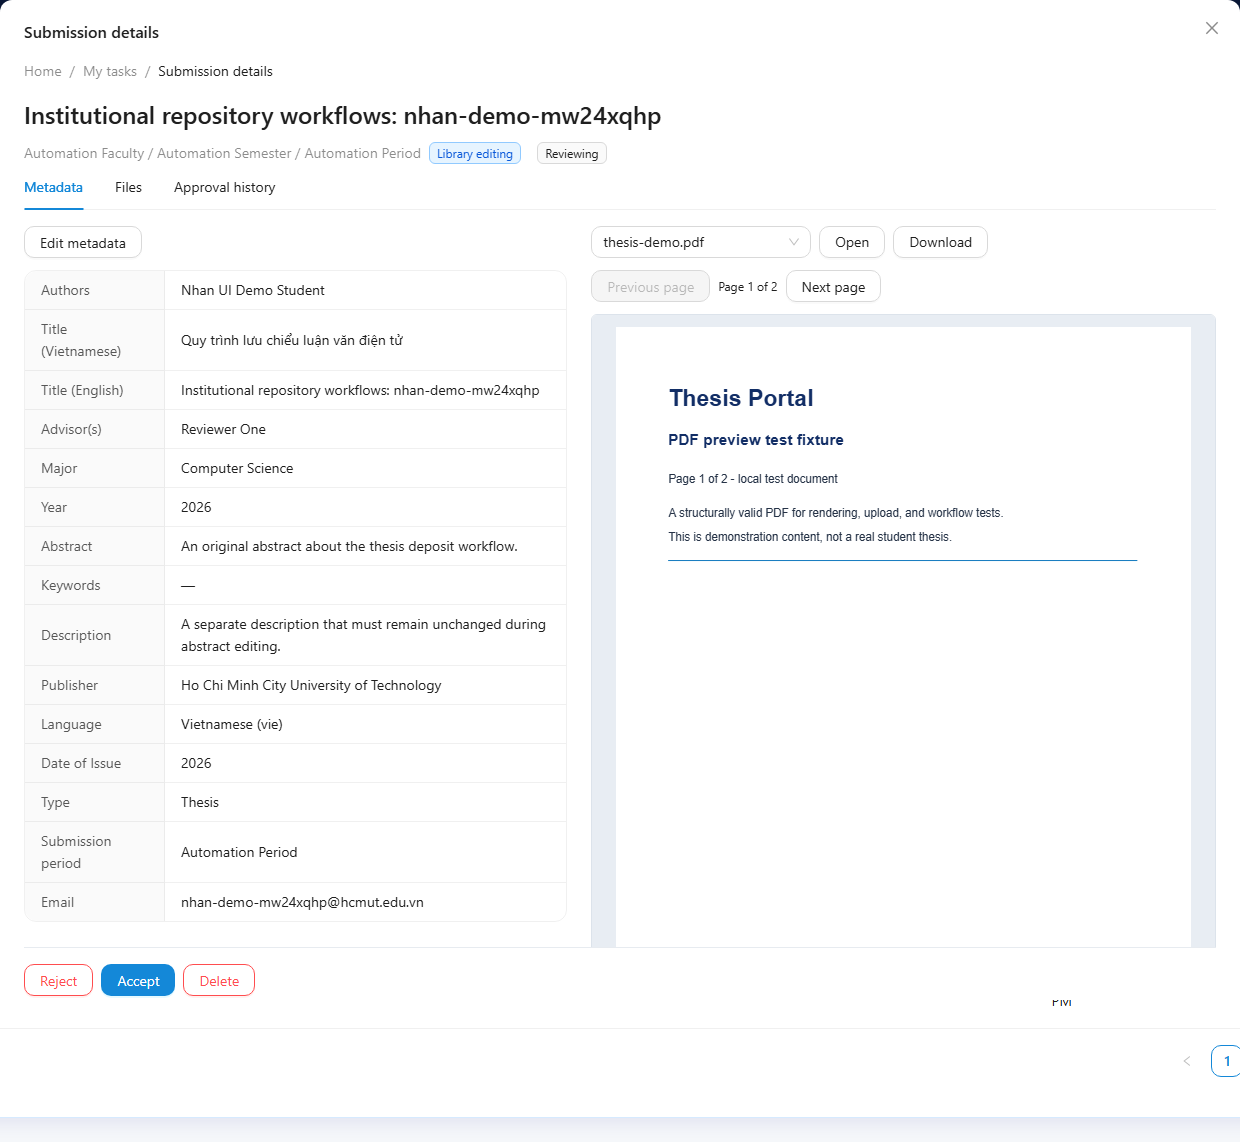
\includegraphics[width=\textwidth,height=0.76\textheight,keepaspectratio]{report-assets/after-editor.png}
\caption{Editor workspace with thesis metadata beside the authenticated PDF.js preview. The document is a two-page test fixture.}
\label{fig:editor-ui}
\end{figure}

\begin{figure}[p]
\centering
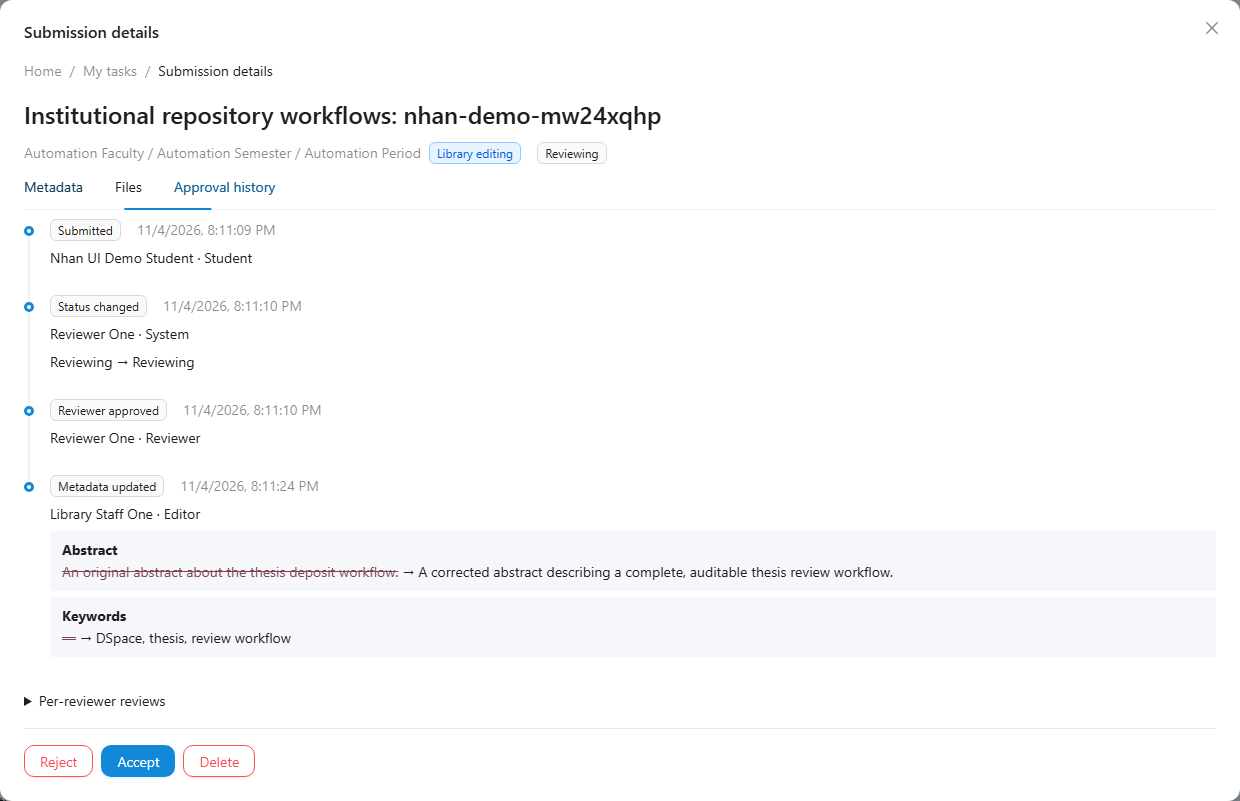
\includegraphics[width=\textwidth,height=0.73\textheight,keepaspectratio]{report-assets/after-history.png}
\caption{Approval history showing actor/role, timestamps, workflow events, and before/after metadata differences.}
\label{fig:history-ui}
\end{figure}

\begin{figure}[p]
\centering
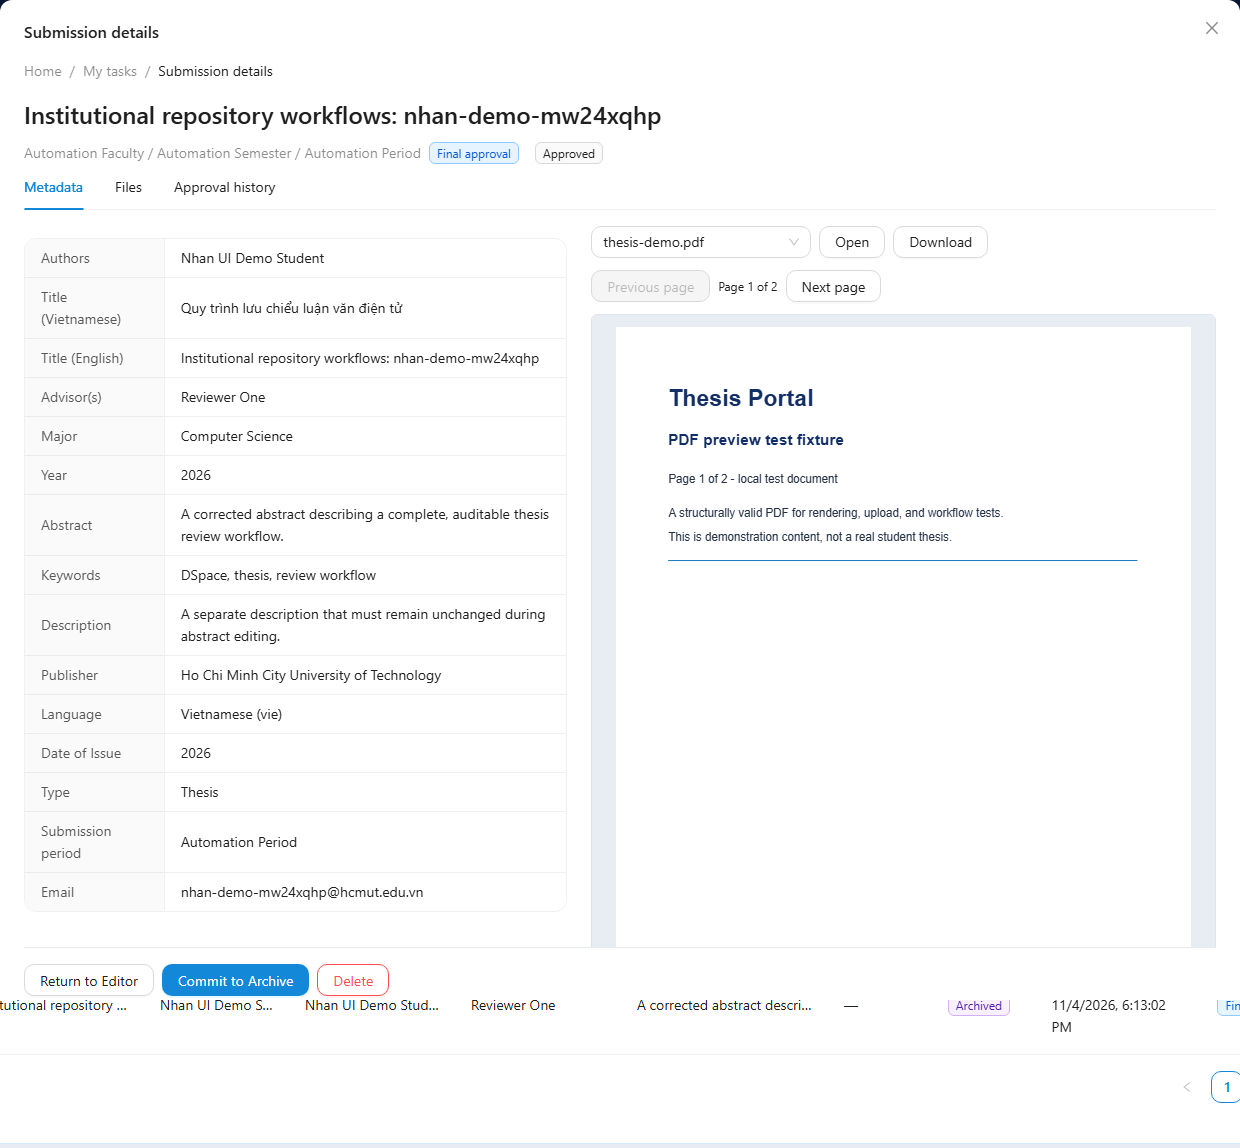
\includegraphics[width=\textwidth,height=0.76\textheight,keepaspectratio]{report-assets/after-final-editor.png}
\caption{Final Editor workspace exposing Return to Editor and Commit to Archive. Portal archival and external publication remain separate.}
\label{fig:director-ui}
\end{figure}

\begin{figure}[p]
\centering
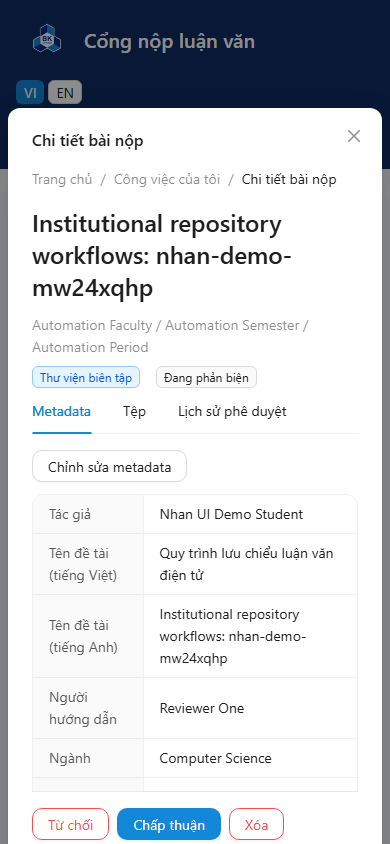
\includegraphics[width=0.43\textwidth,height=0.72\textheight,keepaspectratio]{report-assets/after-mobile-vi.png}
\caption{Narrow-screen Vietnamese review workspace from the local demonstration.}
\label{fig:mobile-ui}
\end{figure}

\begin{figure}[p]
\centering
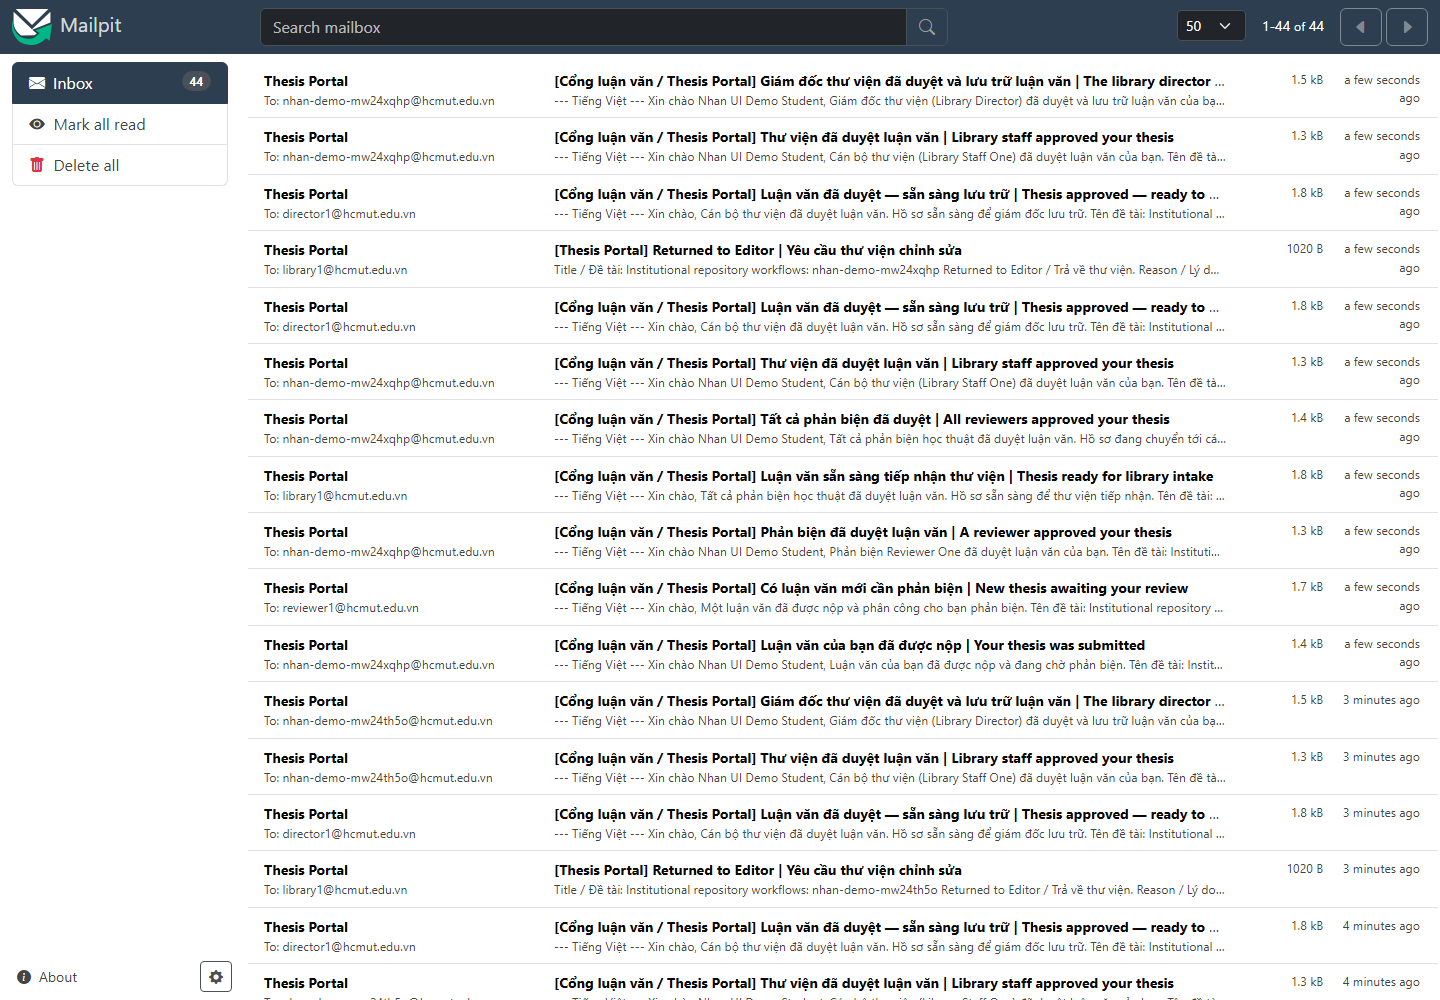
\includegraphics[width=\textwidth,height=0.73\textheight,keepaspectratio]{report-assets/mailpit-inbox.png}
\caption{Mailpit capture of portal-generated workflow messages in the local SMTP demonstration.}
\label{fig:mail-ui}
\end{figure}

\clearpage
\section{Frontend Structure and Maintainability}
The refactor separates the large application, administration, and archive components into the four features described in Chapter~4. The application layer composes public entry points and the shell. Feature providers compose focused controllers for data loading, permissions, selection, mutations, dialogs, workflow actions, and configuration. API functions remain in the owning feature, and a shared transport handles common request behavior.

The legacy \code{App.jsx}, \code{AdminPanel.jsx}, \code{LibraryArchivePanel.jsx}, and workflow paths remain small compatibility adapters. Administration and archive modes use explicit workspace variants. PDF rendering and metadata/history interactions retain local transient state rather than adding those details to a single global controller.

The recorded refactor reduced the legacy entry points from 3,643, 1,722, and 2,080 lines respectively to 1, 25, and 14 lines. Those numbers compare the immediate pre-refactor working source with the compatibility adapters; they do not measure deleted functionality, total code reduction, or a direct line-count comparison with \code{main}. The implementation is distributed across feature modules. Context updates can still rerender consumers, and no rendering-performance improvement is inferred from this restructuring~\cite{refactoring}.

The architecture script checks local import resolution, feature isolation, public entry points, shared-layer direction, direct HTTP usage, and import cycles. The recorded check examined 129 modules. It is a focused guard for literal imports in this codebase, not a complete JavaScript analyzer.

\section{Preparing for HCMUT SSO}
The inherited API uses JWT sessions and supports local/optional Google authentication. The new authentication feature encapsulates restore, login, OAuth callback, logout, and password-related lifecycle behavior. Backend guards continue to consume the authenticated JWT identity independently of individual screen components.

This separation improves the location of a future SSO adapter, but it is not HCMUT SSO integration. An institutional identity contract, callback/logout behavior, account linking, role provisioning, and deployment configuration must be agreed and tested before claiming SSO support.

\chapter{Testing and Evaluation}
\label{ch:evaluation}

\section{Test Strategy and Evidence Boundary}
Evaluation combines source inspection, stored API regression results, SMTP integration results, browser workflows, production-build output, architecture checks, and visual captures. The results below are the branch's recorded executions from 4 November 2026. They are not newly executed application tests during this report revision. Editing this document does not change the test timestamps or convert planned scenarios into observed outcomes.

The environment used local Windows services, PostgreSQL~16, NestJS, Vite/Chromium, and Mailpit. API and browser runs used a disposable \code{thesis_test} database; suites reset it and must run sequentially. The browser harness was corrected to initialize this database before starting NestJS, avoiding termination of active API connections during later global setup. Existing helpers were also aligned with the current read-only faculty selector and explicit English test locale~\cite{validation}.

\section{Recorded Test Results}
\begin{table}[htbp]
\centering\small
\begin{tabularx}{\textwidth}{@{}Y p{0.26\textwidth} r r r@{}}
\toprule
\textbf{Suite} & \textbf{Report time (UTC)} & \textbf{Passed} & \textbf{Failed} & \textbf{Skipped} \\
\midrule
API workflow/regression & 2026-11-04 13:16:36 & 51 & 0 & 0 \\
SMTP/Mailpit integration & 2026-11-04 10:53:32 & 8 & 0 & 0 \\
Playwright browser regression & 2026-11-04 16:49:14 & 12 & 0 & 0 \\
\midrule
Total across these reports & & 71 & 0 & 0 \\
\bottomrule
\end{tabularx}
\caption{Stored local test results. Timestamps are kept in UTC as recorded; 16:49 UTC corresponds to 23:49 on 4 November in Vietnam.}
\label{tab:test-results}
\end{table}

The totals in Table~\ref{tab:test-results} come from the three named reports~\cite{api-evidence,email-evidence,browser-evidence}. Frontend/backend production builds also passed in the stored evidence. The frontend build retained a bundle-size advisory, and the architecture check passed for 129 modules. A separate production-preview check recorded a nonblank two-page PDF, a worker response with HTTP~200, and no page errors. These checks are not additional test cases added to the total of 71.

The earlier report records 56 September tests, including one successful live DSpace publication~\cite{previous-report}. That historical result remains attributed to the previous implementation and environment. It is not included in the current total or used to claim a new live publication test for this branch.

\section{Access Control Testing}
The API suite verifies that reviewers see only assigned submissions, unassigned reviewers cannot decide, and students/library staff cannot invoke academic-review actions. It also checks unauthorized Director and publishing operations. New history tests deny unrelated students and reviewers and reject anonymous access.

Metadata tests deny student/reviewer mutation and reject an Editor save before the active Editor stage or after forwarding to Final Editor. This demonstrates why the active role must be checked in addition to the broad reviewing status. These cases exercise the implemented guards and object checks; they do not establish complete collection-level DSpace permission synchronization or a penetration-test result.

\section{Workflow, Metadata, and Resubmission Testing}
The API cases cover draft creation, required submission metadata, open-period/reviewer requirements, PDF presence/type/size checks, authorized file download, rejection with a reason, and permitted resubmission. Existing academic tests require all assigned reviewers to accept before library intake.

The added metadata cases verify persistence after a partial update, title synchronization, unchanged description, required-field validation, preserved untouched values, no audit event for a no-op, and real before/after differences. The return tests verify a required reason, retained approvals and PDF, movement to Editor and forward again, final portal archival, refusal of Director rejection, earlier-stage refusal, and a stale duplicate return.

\begin{table}[htbp]
\centering\small
\begin{tabularx}{\textwidth}{@{}l Y Y@{}}
\toprule
\textbf{Requirement} & \textbf{Recorded evidence} & \textbf{Observed scope} \\
\midrule
FR-01 & Submission/resubmission API cases; student browser cases. & Valid and invalid submit, rejection/revision, preserved PDF. \\
FR-02, FR-10 & Queue/workspace and navigation browser cases. & Role screens, Home/history, admin/archive loading, mobile Vietnamese. \\
FR-03 & Workspace/PDF stability browser cases; production preview. & Nonwhite rendered pixels, pages, retry, tab/resize/reopen stability. \\
FR-04 & Metadata API cases and Editor browser scenario. & Correct persisted fields, validation, no-op and audit differences. \\
FR-05, FR-06 & Return API cases and workspace browser scenario. & Reasons, failed-input preservation, retained academic approval/files. \\
FR-07 & Archive API/browser cases. & Final-stage guard, confirmation, portal archive, deferred publication. \\
FR-08 & History authorization/API payload and UI timeline checks. & Authorized actors and readable real event data. \\
FR-09 & Eight local mail cases and Mailpit capture. & Relevant recipients/reasons; SMTP failure tolerance. \\
\bottomrule
\end{tabularx}
\caption{Traceability from this report's requirements to existing branch evidence.}
\label{tab:traceability}
\end{table}

Browser tests check persisted values after reload, failed metadata saves, failed return requests with retained reasons, and confirmation before archive. The malformed legacy PDF fixture was replaced with a valid two-page file, and the browser checks actual rendered nonwhite pixels rather than treating a loaded URL as a successful preview. The scrollbar-specific case exercises sustained visibility through page changes, tab changes, resizing, and reopening.

\section{Signature, Print, and Certificate Testing Status}
No cryptographic signing, certificate verification, controlled-print, or signed-receipt test has been executed by this UI package. Table~\ref{tab:planned-sign-tests} retains the essential planned scenarios without assigning invented results.

\begin{table}[htbp]
\centering\small
\begin{tabularx}{\textwidth}{@{}Y Y l@{}}
\toprule
\textbf{Planned case} & \textbf{Required observation} & \textbf{Status} \\
\midrule
Text/scanned/large PDFs & Actual signed output; content preserved; authoritative verification. & Not run \\
Encrypted/corrupt input & Defined signing-input refusal with a recoverable state. & Not run \\
Expired/untrusted/revoked certificate & Defined trust/certificate error and no false success. & Not run \\
Post-signing modification & Integrity check detects the modified signed output. & Not run \\
Unavailable signing service & Retry behavior and no falsely confirmed signature/publication. & Not run \\
Three appearances & Correct placement without unreadable content; cryptographic validity retained. & Not run \\
Print variants and signed receipt & Actual generated files, page/blur rules, receipt verification. & Not run \\
\bottomrule
\end{tabularx}
\caption{Outstanding signing/output tests. These are requirements, not branch test results.}
\label{tab:planned-sign-tests}
\end{table}

The PDF preview's encrypted/invalid-document feedback is separate from these planned signing tests. Likewise, an email stating that a thesis was archived is not evidence of a signed confirmation certificate.

\section{Local Role Demonstration and Email Results}
The recorded demonstration uses local seeded accounts for Student, Reviewer, Library Staff, and Director. It captures an Editor metadata correction, visible differences in history, a Director return, renewed library acceptance, and final portal archival. Its sanitized evidence records preserved description, retained academic approval, a metadata-change event, a return event, and deferred DSpace publication~\cite{demo-evidence}.

The eight SMTP tests cover submission recipients, academic rejection reason, library notification after all reviewers approve, Director notification, library rejection reason, student archival mail, the new library return reason, and successful submission with unreachable SMTP. Mailpit confirms local SMTP capture only. The demonstration does not constitute a trial with real university participants or formal user acceptance testing.

\section{Evaluation Against Goals and Remaining Limits}
The evidence supports the tested portal review/correction flow, protected history, embedded document inspection, and retained administration/archive navigation. The feature refactor is supported by static checks, builds, and browser regression rather than an asserted speed improvement. No code-coverage percentage or load, stress, security, or comprehensive screen-reader result is available.

The local publication tests establish that portal archive is separate, permissions are enforced, invalid publication inputs are rejected, and the archive decision survives an unavailable/missing DSpace configuration. Development placeholder behavior must be distinguished from a real item and bitstream. A current live repository, collection, service account, uploaded PDF, mapped metadata, and returned item/Handle are needed for a fresh publication claim.

Production SMTP, current official deposit-policy text, HCMUT SSO, plagiarism integration, full collection-role synchronization, cryptographic signing, signed certificates, batch processing, and print controls remain unverified or unimplemented as described in the scope. The final Compose seed changes also require a separately recorded fresh-volume startup check. These limits define the next integration work; they do not negate the local workflow results.

\chapter{Conclusion and Future Work}

\section{Achievements}
This project extends the inherited thesis deposit portal with a consistent review workspace and a traceable library correction loop. The current branch places thesis metadata beside an authorized paginated PDF preview, enables validated Editor corrections with actual audit differences, and replaces final-stage rejection to the student with a reasoned return to the prior Editor. It preserves academic approvals and files during that return, protects history access, and retains the separate portal-archive and DSpace-publication operations.

The frontend now separates authentication, submissions, administration, and archive responsibilities through public feature entry points and focused controllers. Existing forms, configuration, bilingual presentation, and archive tools remain available. PDF preview cleanup, failure/retry handling, classic-scrollbar stability, and Home navigation improve the tested interactions. The fresh-database seed and Compose dependency changes support a repeatable demonstration setup, with startup validation still to be recorded for the final revision.

The stored evidence reports 71 passing cases across API, local email, and browser suites on 4 November 2026. These results substantiate the tested local behavior and provide a concrete basis for the next team integrations. They do not establish completion of every phase-1 requirement.

\section{Limitations}
The present work does not implement cryptographic PDF signing, certificate verification, signed deposit confirmation certificates, signature appearances, print restrictions, or batch signing. Director archival currently records a portal outcome and defers repository publication. Current live DSpace publication and production mail delivery require further validation. Supplied deposit guidance still needs confirmation against current institutional policy.

The recorded tests use local demonstration accounts and fixtures. Formal acceptance with library staff and students, comprehensive accessibility evaluation, production security review, and performance/load measurement remain outside the collected evidence. The previous report's live repository result is historical prior-work evidence, not a current-branch integration result.

\section{Remaining Phase-1 Work}
The next phase-1 integration should establish the signing service contract and signer identity, produce and verify real signed PDFs, define recovery states, and connect the output to archival/publication without falsely reporting success. It should then add the three signature appearances, signed confirmation certificates, print variants, and batch handling with dedicated output and failure tests.

The team should validate DSpace publication against the intended repository and collection, record item/bitstream/metadata results, obtain the real Handle where provided, and send any promised repository link only after it is available. Collection-level group/role behavior and production email recipients/settings need corresponding evidence. A fresh-volume Docker startup should confirm initialization, seed gating, shared PDF files, and startup ordering for the final Compose revision.

\section{Phase 2 Directions}
Future work includes HCMUT SSO, plagiarism-assessment integration, and support for additional document types such as scientific reports and dissertations. SSO requires institutional account mapping and role provisioning. Plagiarism integration requires an explicit request/result contract and an agreed influence on review decisions. New document types require adapted metadata and workflows rather than a title change alone. A later printing stage can reuse an agreed processing contract once the signing/output pipeline exists.

\begin{thebibliography}{99}
\addcontentsline{toc}{chapter}{References}

\bibitem{previous-report}
Ngo Nhat Tuan, \emph{Developing a Web-Based System for Submitting and Archiving Undergraduate Theses Integrated with the DSpace Digital Library}, capstone project report, HCMUT, September 2026. Supplied file: \path{HK253-DATN-028_2213774.pdf}. Used for attributed baseline design and historical evaluation.

\bibitem{source-snapshot}
Project repository, \code{main} at \code{4f7a73df} and \code{UI-build} at \code{3d97faf3}, local source comparison inspected for this revision, 5 November 2026. Relevant areas: \path{backend/src/submissions}, \path{backend/src/reviews}, \path{backend/src/archive}, \path{backend/src/mail}, \path{frontend/src/features}, and \path{docker-compose.yml}.

\bibitem{ui-report}
Nguyen Phuc Nhan, \emph{Thesis Portal UI: weeks 1--6 submission}, 4 November 2026. Repository artifact: \path{frontend/docs/report.md}.

\bibitem{ui-research}
Project UI research and requirements notes, recorded 4 November 2026. Repository artifact: \path{frontend/docs/research-and-requirements.md}; supplied policy summary: \path{docs/quy-dinh-nop-luu-chieu-thu-vien.md}. Public source status and policy-verification limits are recorded in the research notes.

\bibitem{api-contract}
Project frontend workflow API contract and flow diagrams. Repository artifacts: \path{frontend/docs/api-contract.md} and \path{frontend/docs/flows.md}.

\bibitem{refactoring}
Project frontend architecture/refactor record and dated check results, 4 November 2026. Repository artifacts: \path{frontend/docs/refactoring.md} and \path{frontend/docs/evidence/refactoring.json}.

\bibitem{validation}
Project validation scope, environment, commands, and remaining integrations. Repository artifact: \path{frontend/docs/validation.md}.

\bibitem{api-evidence}
Stored API regression report, 4 November 2026, 13:16:36 UTC; 51 passed. Repository artifact: \path{frontend/docs/evidence/api-report.md}.

\bibitem{email-evidence}
Stored email integration report, 4 November 2026, 10:53:32 UTC; 8 passed. Repository artifact: \path{frontend/docs/evidence/email-report.md}.

\bibitem{browser-evidence}
Stored Playwright report, 4 November 2026, 16:49:14 UTC; 12 passed. Repository artifact: \path{frontend/docs/evidence/playwright-report.md}.

\bibitem{demo-evidence}
Sanitized local demonstration evidence and screenshots, 4 November 2026. Repository artifacts: \path{frontend/docs/evidence/demo-evidence.json} and \path{frontend/docs/screenshots/}. Images in this report are copied from these existing captures.

\bibitem{pdf-stability}
Stored PDF stability and production-preview observations, 4 November 2026. Repository artifacts: \path{frontend/docs/evidence/pdf-preview-stability.json} and \path{frontend/docs/evidence/production-preview.json}.
\end{thebibliography}

\appendix
\chapter{Implementation and Evidence Map}
This appendix links report claims to repository artifacts. Paths are relative to the project root and describe the snapshot identified in the abstract.

{\small
\begin{longtable}{@{}>{\raggedright\arraybackslash}p{0.30\textwidth} >{\raggedright\arraybackslash}p{0.65\textwidth}@{}}
\toprule
\textbf{Responsibility} & \textbf{Source or evidence} \\
\midrule
\endfirsthead
\toprule
\textbf{Responsibility} & \textbf{Source or evidence} \\
\midrule
\endhead
\bottomrule
\endfoot
Editor persistence and history access & \path{backend/src/submissions/submissions.service.ts} \\
Director return/archival and locked stage checks & \path{backend/src/reviews/reviews.service.ts} \\
Return notification & \path{backend/src/mail/workflow-mail.service.ts} \\
Shared workspace and role actions & \path{frontend/src/features/submissions/workflow/ReviewWorkspace.jsx} \\
Authenticated document fetch & \path{frontend/src/features/submissions/workflow/PdfPreview.jsx} \\
Canvas/page rendering & \path{frontend/src/features/submissions/workflow/PdfCanvas.jsx} \\
Metadata form and audit timeline & \path{frontend/src/features/submissions/workflow/MetadataEditor.jsx}\newline \path{frontend/src/features/submissions/workflow/ApprovalHistory.jsx} \\
Application composition/session shell & \path{frontend/src/app/PortalApp.jsx}\newline \path{frontend/src/app/PortalShell.jsx} \\
Feature architecture guard & \path{frontend/scripts/check-architecture.mjs} \\
Fresh-database demo seed & \path{backend/scripts/seed-demo.cjs}\newline \path{db/init/002_demo_bootstrap.sql} \\
Workflow/API regression cases & \path{backend/test/workflow-ui.e2e-spec.ts} \\
Workspace and PDF regression cases & \path{playwright/workspace.spec.ts}\newline \path{playwright/pdf-stability.spec.ts} \\
Home/admin/archive navigation cases & \path{playwright/home-navigation.spec.ts}\newline \path{playwright/refactor-navigation.spec.ts} \\
Editable use-case and wireframe sources & \path{frontend/docs/diagrams/use-cases.puml}\newline \path{frontend/docs/wireframes.html} \\
\end{longtable}
}

\end{document}
